\documentclass{article}\usepackage[]{graphicx}\usepackage[]{color}
% maxwidth is the original width if it is less than linewidth
% otherwise use linewidth (to make sure the graphics do not exceed the margin)
\makeatletter
\def\maxwidth{ %
  \ifdim\Gin@nat@width>\linewidth
    \linewidth
  \else
    \Gin@nat@width
  \fi
}
\makeatother

\definecolor{fgcolor}{rgb}{0.345, 0.345, 0.345}
\newcommand{\hlnum}[1]{\textcolor[rgb]{0.686,0.059,0.569}{#1}}%
\newcommand{\hlstr}[1]{\textcolor[rgb]{0.192,0.494,0.8}{#1}}%
\newcommand{\hlcom}[1]{\textcolor[rgb]{0.678,0.584,0.686}{\textit{#1}}}%
\newcommand{\hlopt}[1]{\textcolor[rgb]{0,0,0}{#1}}%
\newcommand{\hlstd}[1]{\textcolor[rgb]{0.345,0.345,0.345}{#1}}%
\newcommand{\hlkwa}[1]{\textcolor[rgb]{0.161,0.373,0.58}{\textbf{#1}}}%
\newcommand{\hlkwb}[1]{\textcolor[rgb]{0.69,0.353,0.396}{#1}}%
\newcommand{\hlkwc}[1]{\textcolor[rgb]{0.333,0.667,0.333}{#1}}%
\newcommand{\hlkwd}[1]{\textcolor[rgb]{0.737,0.353,0.396}{\textbf{#1}}}%
\let\hlipl\hlkwb

\usepackage{framed}
\makeatletter
\newenvironment{kframe}{%
 \def\at@end@of@kframe{}%
 \ifinner\ifhmode%
  \def\at@end@of@kframe{\end{minipage}}%
  \begin{minipage}{\columnwidth}%
 \fi\fi%
 \def\FrameCommand##1{\hskip\@totalleftmargin \hskip-\fboxsep
 \colorbox{shadecolor}{##1}\hskip-\fboxsep
     % There is no \\@totalrightmargin, so:
     \hskip-\linewidth \hskip-\@totalleftmargin \hskip\columnwidth}%
 \MakeFramed {\advance\hsize-\width
   \@totalleftmargin\z@ \linewidth\hsize
   \@setminipage}}%
 {\par\unskip\endMakeFramed%
 \at@end@of@kframe}
\makeatother

\definecolor{shadecolor}{rgb}{.97, .97, .97}
\definecolor{messagecolor}{rgb}{0, 0, 0}
\definecolor{warningcolor}{rgb}{1, 0, 1}
\definecolor{errorcolor}{rgb}{1, 0, 0}
\newenvironment{knitrout}{}{} % an empty environment to be redefined in TeX

\usepackage{alltt}
\usepackage[stable]{footmisc}
\usepackage{fullpage}
\usepackage{setspace}
\usepackage[]{graphicx}
\usepackage[]{color}
\usepackage[OT1]{fontenc}
\usepackage{amsthm,amsmath,amsfonts}
\usepackage{natbib}
\usepackage[colorlinks,citecolor=blue,urlcolor=blue]{hyperref}
\usepackage{bm}
\usepackage{subcaption}
\usepackage{graphicx}
\usepackage{multirow}
\usepackage{xr}
\usepackage{tikz}
\usepackage{authblk}
\usepackage[section]{placeins}
%\usepackage{endfloat}

\doublespacing

\newcommand{\yti}{Y_{Ti}}
\newcommand{\yci}{Y_{Ci}}
\newcommand{\uti}{U_{Ti}}
\newcommand{\uci}{U_{Ci}}
\newcommand{\hcont}{\bar{h}}
\newcommand{\etat}{\hcont(1)}
\newcommand{\hcontti}{\hcont(1)_{i}}

\newcommand{\mti}{\bar{m}_{Ti}}
\newcommand{\byt}{\bm{Y_T}}
\newcommand{\byc}{\bm{Y_C}}
\newcommand{\bmt}{\bm{\bar{m}_T}}
\newcommand{\bmi}{\bm{m}_i}
\newcommand{\bsi}{\bm{s}_i}

\newcommand{\EE}{\mathbb{E}}

% see
% https://tex.stackexchange.com/questions/42726/align-but-show-one-equation-number-at-the-end
\newcommand\numberthis{\addtocounter{equation}{1}\tag{\theequation}}


\newenvironment{ass}[2][Assumption:]{\begin{trivlist}
\item[\hskip \labelsep {\bfseries #1}\hskip \labelsep {\bfseries #2}.]}{\end{trivlist}}

\def\independenT#1#2{\mathrel{\rlap{$#1#2$}\mkern2mu{#1#2}}}
\newcommand\independent{\protect\mathpalette{\protect\independenT}{\perp}}

\newcommand{\indicator}[1]{\mathbf{1}_{\left[ {#1} \right] }}




\renewenvironment{knitrout}{\begin{singlespace}}{\end{singlespace}}

\title{Student Log-Data from a Randomized Evaluation of Educational
  Technology: A Causal Case Study}



\author[1]{Adam C Sales}
\author[2]{John F Pane}
\affil[1]{University of Texas, Austin, TX}
\affil[2]{RAND Corporation, Pittsburgh, PA}

%\affiliation{University of Texas College of Education and RAND Corporation}







\IfFileExists{upquote.sty}{\usepackage{upquote}}{}
\begin{document}
\maketitle

\section{Introduction}
From 2007 through 2010, the RAND corporation
conducted one of the first effectiveness trials awarded through
competitive grant programs sponsored by the US Department of
Education's Institute of Education Sciences.  The randomized
controlled trial (RCT) was
designed to estimate the effect of school-wide adoption of the
Cognitive Tutor Algebra I (CTA1) curriculum, whose centerpiece is a
computerized ``tutor'' that uses cognitive science principles to teach
Algebra I \citep{anderson1985intelligent}.
The study \citep{pane2014effectiveness} found no effects in its first year, but in
the second year of implementation students in high schools randomized to
the CTA1 condition outperformed the control group on the posttest by a fifth of a
standard deviation.

Over the course of the CTA1 study, the software administrators
gathered computer log data for students in the treatment group.
They assembled a dataset that records which problems each student
worked, along with timestamps, the numbers of hints requested, and the
number of errors committed for each problem.
Log data from experiments like this present an unprecedented
opportunity for education researchers:
to use the fine-grained and rich data to
help understand how, why, and when educational technology works.

Along the same lines, log data presents a challenge, since it differs in
structure and size from the type of data commonly encountered in
studies of causal mechanisms.
While statistical models of log data are nearly as old as the data itself
\citep[e.g.][]{corbett1994knowledge}, data from an RCT differs in
two principal ways from more traditional domains.
RCTs feature randomization of treatment assignment, and a posttest
(or some other outcome) administered to both users and non-users.
These factors allow for causal modeling.

As educational technology booms, so do RCTs in the mold of the RAND
CTA1 study. A recent systematic review \citep{escueta2017education} cites 29
published reports of RCTs of ``computer assisted learning'' programs,
all but one of which was published since 2001. We are aware of
numerous other such RCTs planned or ongoing. The current case-study is
about the use of hints in CTA1, but the huge variation in products
under study, each with their own unique designs, opens a wide set of opportunities to understand how features of those
products drive their effects. As one example, RAND is recently
completed an efficacy study of a different algebra tutoring system,
ALEKS. When students begin working on a particular topic in ALEKS, the
system first presents instructional material, followed by problem
solving activities, and then, if students are unsuccessful at solving
the problems, more instructional material. Some students diligently
read the initial instructional material while others skip it and dive
directly into problem solving. Is skipping the material a productive
strategy for students in terms of learning algebra, or should ALEKS be
redesigned to prevent such skipping? Researchers should not stop at
estimating overall average treatment effects, but make use of the
wealth of log data that these RCTs produce automatically, as a
bi-product. Our hope is that this paper can serve as a starting point
for researchers interested in mining this rich resource.

This paper will illustrate three approaches to this type of research
using log data from the CTA1 study---specifically, data on students' use
of hints within the software.
The first approach discards the control group, and analyzes
hint-requesting in the treatment group as an observational study,
using a matching design
\citep[c.f.][]{rosenbaum2002observational}. The
second approach applies the framework of causal mediation analysis
\citep{vanderweele2015explanation,hong2015causality,imai2011unpacking} to estimate the role of
hint-requesting in the overall CTA1 treatment effect. However, since
students in the control group were unable to request hints, not all
mediational estimands are identified, and estimation methods must be
modified.
Finally, we conduct a principal stratification analysis
\citep{frangakis} to learn if students requesting different amounts of
hints experienced different treatment effects.

Our intention is to develop, demonstrate, and contrast these three
approaches to modeling log data.
A rich, and often polemic, literature surrounds principal
stratification and mediation analysis
\citep[e.g.][]{rubin2004direct,vanderweele2011principal,pearl2011principal,mealli2012refreshing,vanderweele2012comments}.
\citet{vanderweele2008simple}, \citet{jo2008causal} and others have
derived formal equivalencies between parameters under certain
conditions.
Our contribution will build on this literature in two ways: first, by
providing a detailed demonstration and comparison of matching, mediation analysis,
and principal stratification on the same dataset, and second by
focusing on the applicability of these three methods in the specific
context of studying implementation data from an randomized
experiment studying educational technology (EdTech).

After a brief overview of the three causal approaches,
the next section will provide background for the case-study,
describing the CTA1 curriculum, the RAND study, and our focus on
hints.
The following three sections will present the observational study,
causal mediation, and principal stratification approaches to the hint
data.
Section \ref{sec:synthesis} will compare the three methods directly,
and discuss how they may be applied to data from other educational
technology RCTs.
Section \ref{sec:conclusion} will conclude.

\subsection{Brief Overview of Three Causal Approaches}
\begin{figure}
\centering
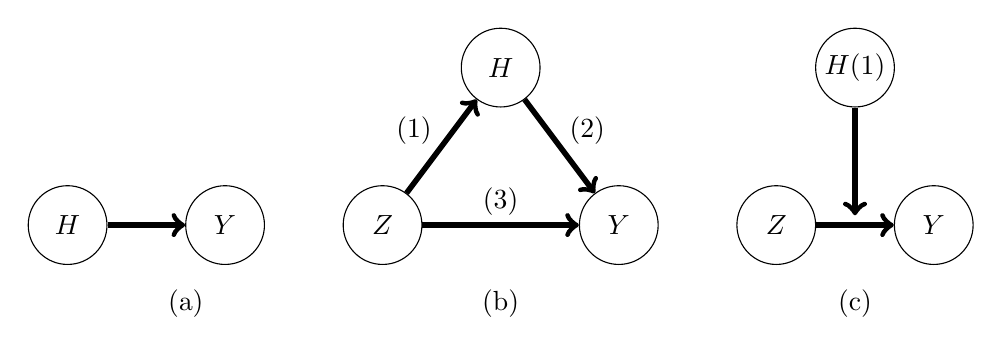
\begin{tikzpicture}[scale=1,transform shape]
	%\draw[help lines] (0,0) grid (15,3);
	\node[draw,shape=circle, inner sep=0pt,minimum size=1cm] (z) at (1,0) {$H$};
	\node[draw,shape=circle, inner sep=0pt,minimum size=1cm] (y) at +(0:3){$Y$};
	%\node[draw,shape=circle, inner sep=0pt,minimum size=1cm] (x) at (2.5,3.5){$X$};
	%\draw[->,line width=2pt](x)--(z);
	%\draw[->,line width=2pt](x)--(y);
	\draw[->,line width=2pt](z)--(y);
	\node at (2.5,-1) {(a)};

	\node[draw,shape=circle, inner sep=0pt,minimum size=1cm] (z) at (5,0) {$Z$};
	\node[draw,shape=circle, inner sep=0pt,minimum size=1cm] (y) at +(8,0){$Y$};
	\node[draw,shape=circle, inner sep=0pt,minimum size=1cm] (m) at (6.5,2){$H$};
	\draw[->,line width=2pt](z)--(m);
	\draw[->,line width=2pt](m)--(y);
	\draw[->,line width=2pt](z)--(y);
	\node at (5.4,1.2) {(1)};
	\node at (7.6,1.2) {(2)};
	\node at (6.5,.3) {(3)};
	\node at (6.5,-1) {(b)};

        \node[draw,shape=circle, inner sep=0pt,minimum size=1cm] (z) at (10,0) {$Z$};
	\node[draw,shape=circle, inner sep=0pt,minimum size=1cm] (y) at +(12,0){$Y$};
        \node (mid) at (11,0) {};
        \node[draw,shape=circle, inner sep=0pt,minimum size=1cm] (h)
        at (11,2) {$H(1)$};
	%\node[draw,shape=circle, inner sep=0pt,minimum size=1cm] (x) at (2.5,3.5){$X$};
	%\draw[->,line width=2pt](x)--(z);
	%\draw[->,line width=2pt](x)--(y);
	\draw[->,line width=2pt](z)--(y);
        \draw[->,line width=2pt](h)--(mid);
	\node at (11,-1) {(c)};

\end{tikzpicture}
\caption{A schematic representation of three causal models for
  log data: (a) an observational study estimating the effects of hints
  $H$ on posttest scores $Y$, (b) a mediation analysis estimating
  natural direct effects of treatment assignment $Z$ on $Y$ and
  indirect effects mediated by $H$, and (c) principal stratification.}
\label{mediationFig}
\end{figure}

Figure \ref{mediationFig} is a schematic representation of the three
approaches to causal modeling of log data that we will discuss in this
paper.
First, an observational study to estimate the effect of hint usage $H$
on posttest scores $Y$, is represented by figure (a).
This approach, which we will discuss in Section
\ref{sec:observational}, discards the control group from the RCT and
uses techniques from observational studies to determine if and how requesting
a greater number of hints affects posttest scores.
For the sake of illustration, we will use techniques similar to those
discussed in \citet{rosenbaum2002observational},
 \citet{hansen2009b}, and \citet{ho:etal:2007}, combining a propensity
 score matching design with methods for analyzing experiments and
 parametric modeling.
The conceptual and methodological issues we will discuss extend to
other covariate control methods as well.

Next, as represented in Figure (b), we will conduct a mediation
analysis, estimating natural
indirect effects of CTA1 treatment assignment $Z$, as mediated by
$H$. That is, we will estimate the component of $Z$'s effect on $Y$ that comes about
due to $Z$'s effect on $H$---path (1)---and $H$'s effect on $Y$, path
(2).
Notice that path (2) is identical to figure (a)---the effect of $H$ on
$Y$.
We will use this equivalence to estimate and interpret indirect
effects.
As part of the mediation analysis, we will also estimate path (3), the
natural direct effect of $Z$ on $Y$---that is, the component of $Z$'s
effect on $Y$ that is not due to hints $H$.

Finally, we will estimate a principal stratification model, as represented in Figure
(c).
In the principal stratification analysis, we do not model $H$ as an
intervention that could, in theory, be randomized.
Instead, we posit a variable ``$H_i(1)$,''  subject $i$'s penchant for
requesting hints \emph{if} $i$ is assigned to the treatment
condition.
Unlike $H$, $H(1)$ is well defined (if
unobserved) for all participants in the RCT.
Principal stratification treats $H(1)$ as an effect moderator or
interaction variable: $H(1)$ does not affect $Y$, but the effect of
$Z$ on $Y$ may vary as a function of $H(1)$.
This analysis will largely follow the method of \citet{aoas}, which in
turn built heavily on \citet{schwartz2011bayesian} and
\citet{jin2008principal}.

All three of these approaches are designed to model intermediate
variables---those variables, like hint usage,
that were possibly affected by $Z$ but were measured prior to $Y$.
Though they were developed for more traditional data scenarios, the
novel scenario of computer log data from an educational technology RCT
presents new and interesting challenges and opportunities.

\section{Case Study: The Role of Hints in the Cognitive Tutor Effect}

\subsection{The Cognitive Tutor}
CTA1 is one of a series of complete mathematics curricula developed by
Carnegie Learning, Inc., which include both textbook materials and an
automated computer-based Cognitive Tutor
\citep{anderson1995cognitive,pane2014effectiveness}.

The computerized tutor was originally built to test the ACT and ACT-R
theories of cognition \citep{anderson2013architecture}.
These are elaborate theories that describe, among other things, the necessary components of
cognitive skills in, say, mathematics or computer programming, and the
process of acquiring those skills.
The Algebra I tutor guides students through a sequence of Algebra I
problems nested in sections within units, and organized by the specific sets of skills they require.
Students move through the curriculum as the tutor's internal learning
model determines that they have mastered the requisite skills.


\subsection{The Role of Hints\footnote{This subsection draws heavily
  on comments from an anonymous reviewer.}}
Students using the Cognitive Tutor Algebra software work algebra
problems on a computer.
Each problem in the software is associated with a set of skills that
the student must master, and a path (or set of paths) to solving the
problem.
As soon as a student errs in working through a problem---that is, departs from one of the
solution paths---the
software shows the student an error message.
This feedback is tailored to the specific mistake, and
designed to guide the student back to a correct solution path.
Similarly, when a student gets stuck, and is unable to determine the
next step in solving the problem, he or she can ask for a hint.
Like the error feedback, these hints are tailored to the specific
algebra skills corresponding to the next step on the solution path.
Thus, hints and error feedback are crucial aspects of the tutor's
pedagogy.

There are good reasons to believe that the availability of
hints---help on demand---may increase student learning, but there is
also reason to be skeptical \cite[See][for an overview of the theory]{aleven2016help}.
First of all, as, e.g., \citet{anderson1995cognitive} points out, ``if
students never receive help of any sort, they are in danger of becoming
permanently stuck on some problem'' (p. 190).
That is, hints give students who are stuck a way to continue working.
Hints may also boost learning by ``helping students identify relevant features in
problems'' \citep[][p. 6]{aleven2016help},  that is, point students
towards aspects of the problem that are ``most important for the goals
of learning'' \citep[][p. 782]{koedinger2012knowledge}.
Hints can help improve students' self-awareness and
problem-solving strategy, such as by clarifying which skills they have
and have not mastered.

Most problems are associated with several hints, arranged in a
sequence so that a student who remains stuck after one hint may
request another.
The last hint in the sequence will show a complete solution to the
problem---essentially showing students a worked example, which can be an
effective tool for learning \citep[e.g.][]{sweller1985use}.

On the other hand, all of these theoretical mechanisms rely on
students to play their part.
In order for hints to be instructive, students need to reflect on
their content in productive ways.
This suggests that hints may be helpful for some students but not for
others.
In the same vein, hints need to be well-designed in order to be
effective \citep{mckendree1990effective}, so some hints may be more
helpful than others.

Hints may even be harmful: as \citet{koedinger2007exploring} put it
(p. 241),
``many lines of research and theory suggest the importance of \dots
withholding information from students so that they can exercise, test,
or reason toward new knowledge on their own.''
\citet{paas1994variability} interpret this dilemma in terms of balancing
``cognitive load,'' that is, optimally allocating a student's
attention to the most relevant aspects of a problem.

The empirical literature on the value of hints in intelligent tutors
is mixed \citep[see][for a summary]{goldin2012learner}.
\citet{anderson1995cognitive} compared the performance of students
randomly assigned to different versions of the Cognitive Tutor with
different feedback structures, and found that students who were able
to request hints finished the lesson faster than those who were not,
but could not detect an effect on learning.
\citet{singh2011feedback} used a similar design, comparing two
versions of the ASSISTments intelligent tutor, one in which hints and
immediate error messages were available, and one which did not provide
feedback. Students in the feedback condition showed larger gains on a
posttest, though it is unclear whether these gains were due to hints
or error feedback.
On the other hand, \citet{beck2008does} and \citet{goldin2012learner}, did not randomize hint
availability, but instead used statistical models to control for
observed confounding.
Both papers used students' subsequent performance within the tutor to
estimate hint effects.
\citet{beck2008does} found conflicting results using different
analytical methods to control for confounding.
\citet{goldin2012learner} investigated two sources of heterogeneity in
the effect of a hint request: by student and by the ``level'' of the
hint (the first, second, or final hint available for a given problem).
They found that, indeed, the effect of asking for a hint varies
between students, but on average it is negative for the first two
hints requested on a problem, but positive for the final hint.

\subsection{Measuring Hint Usage in the CTA1 Data}
%\marginpar{make sure this makes sense before ``Data'' section}
Unlike previous studies of hint usage, the CTA1 study was not designed
to estimate the effect of hint usage; its purpose was to estimate the
effect of CTA1 as a package, including the associated textbook and
recommended classroom practices.
Access to the full CTA1 curriculum was randomized, rather than any
specific aspect of usage, and effectiveness was measured with a
standardized posttest covering a broad range of Algebra I skills.
In this regard, the CTA1 study is similar to other large-scale
evaluations of educational technology which do not randomize usage but
do include a posttest.

The CTA1 study was of a much longer duration than
any of the studies of hint effects we are aware of: students had access to the tutor for an entire
school year before the posttest.
This factor allows for much more data for each student than shorter
studies, as well as more variability in the types of problems and
contexts in which students may request hints.
This variability, in turn, allows researchers to fit flexible models
and ask nuanced questions about hint usage, for instance, exploring differing
patterns of usage among different students.
This sort of analysis is beyond the scope of the current study, which
focuses on comparing and contrasting causal modeling approaches for
these data.

For the current purpose, we narrow down the type
of hint data we model to align with our research focus.
Since our posttest measured Algebra I skills, we only
considered worked problems from the Algebra I curriculum.
Next, although \citet{goldin2012learner} demonstrated the importance
of hint level, our focus is on the overall average effect of
requesting any hints; therefore, the variable measuring a student's
hint request on a problem was set to one if the student requested any
hints on that problem, and zero otherwise.
% (More mundanely, we do not have access to data
% describing the number of hints available for every problem, which
% would hinder interpretation of any other measure of hint usage.)

Lastly, any observational study of hint usage must contend with the
fact that students are unlikely to request hints on problems that they
already know how to solve.
Hence, any measure of hint usage is necessarily also a measure of
student ability---students who know more algebra will almost certainly
request fewer hints.
This leads to two related problems: first, student ability
confounds any statistical relationship between hint request frequency
and posttest scores.
Secondly,
a student's decision to request a hint implies both that she
found the problem at least somewhat difficult, and that, in this case,
she responded to that difficulty by requesting a hint.
Our interest is in the second implication, not the first.
Conversely, the significance of a student's decision to forgo a hint
depends in part on how challenging he or she finds the problem.
Hint request frequency combines students' hint requests (or non-requests) from both
problems they find challenging and trivial, so is a poor measure of
students' disposition to use the hint feature.

Ideally, we would solve this problem by only including data on
problem-student pairs in which the problem was challenging to the
student.
Of course, no direct measure of problem challenge is available.
Instead, we considered a problem to be challenging if the student
either requested a hint or made an error on that problem.
Then, let
\begin{equation*}
\bar{h}_i=\frac{\text{\# problems on which }i\text{ requested a
    hint}}{\text{\# problems on which }i\text{ either requested a hint
    or made an error}}
\end{equation*}
measure hint frequency.

This measure is inversely related to the ratio of the percentage (of
all
problems) a student makes an error without having requested a hint,
to the percentage of problems a student requests a hint.%
\footnote{Technically, if $h$ is the event that a student requests
a hint on a problem and $e$ is the event that the student makes
an error, then $Pr(h|h\text{ or }e)=1/\{1+Pr(e\text{ and not }h)/Pr(h)\}$.}
Making an error on a problem without having requested a hint reflects
a hesitance to request a hint when one might have been warranted.
$\bar{h}$ ignores the class of challenging problems on which students
are challenged and figure the answer out (or guess correctly) without
requesting a hint.
This class of problems is inherently interesting to our question;
however, it is unidentified.

\subsubsection{Dichotomizing Hint Usage}\label{sec:dichotomizingHintUsage}
The observational study and mediation analysis below require a dichotomous measurement of hint usage: is a
student a high or low hint user?
To this end, we dichotomize $\bar{h}$ by comparing it to a cutoff value, so
that $H_i=\indicator{\bar{h}_i>c}$, where $\indicator{x}=1$ if $x$ is true
and 0 otherwise.

To choose $c$, we first fit a modified Rasch mixture model
\citep{rasch} to hint request data.
Specifically, we modeled the probability of a hint request in each problem
$p$, worked by student $i$, as
\begin{equation*}\label{eq:rasch}
Pr(h_{ip})=logit^{-1}(\eta_i+\delta_{s[p]})
\end{equation*}
where $h_{ip}$ is the event that student $i$ requests a hint on
problem $p$, $\eta_i$ is a student parameter, $\delta_{s[p]}$ is a
section-level parameter for $s[p]$, the section that problem $p$ was
drawn from, and $logit^{-1}(x)=\{1+exp(-x)\}^{-1}$ is the inverse logit
function.
Typically, the student parameter $\eta_i$ measures student ability;
here, instead, it measures a student's proclivity to request a hint.
The typical Rasch model includes a problem-level ``difficulty'' parameter, but in our
dataset many problems were worked by very few students, so problem
level parameters would be hard to estimate.
Instead, we included the section-level parameter $\delta_{s[p]}$,
which measures the extent to which students tend to request hints on
problems in section $s$.
This essentially assumes that all problems within each section are equally
likely to elicit a hint.

Then, in order to dichotomize hint request behavior, we modeled
student effects $\eta$ as
\begin{equation}\label{eq:mixture}
\eta\sim
p_0\mathcal{N}(\mu_0,\sigma_0)+(1-p_0)\mathcal{N}(\mu_1,\sigma_1)
\end{equation}
and constrained $\mu_0<\mu_1$.
This mixture model clusters students into two categories: high hint
users have $\eta$ drawn from a normal distribution with mean $\mu_1$
and standard deviation $\sigma_1$, and low hint users have $\eta$
drawn from a normal distribution with mean $\mu_0$ and standard
deviation $\sigma_0$.

Our main parameter of interest here is $p_0$, the proportion of
students who are low hint users.
We estimated $p_0\approx$0.7,
classifying 30\% of students as
high hint users, so we chose $c$ as the
70th percentile of $\bar{h}$,
approximately 0.6.
This definition agreed with the model's classification (based on
$\eta$ as opposed to $\bar{h}$ in
approximately 93\% of cases.

The Rasch model for hint usage \eqref{eq:rasch}, but not the mixture
model \eqref{eq:mixture} will play an important role in the principal
stratification analysis of Section \ref{sec:principalStratification}.



\subsection{Data}\label{sec:data}

\citep{pane2014effectiveness} estimated effects separately in middle
schools and high schools in each the first two years of the RCT; the
only statistically significant treatment effect was in the high school
sample in the second year.
Since our goal was to better understand the CTA1
treatment effect, we focused our analysis on data from high school students in
the second year of the CTA1 trial, for whom the treatment effect was
most evident.

We merged data from two sources: computerized log data gathered by
Carnegie Learning, and covariate, treatment and outcome data gathered by RAND.

The log data lists the problem name, section, and unit of
each problem, the numbers of hints requested and errors committed, and time-stamps.
Log data were missing for some students, either because the log files
were not retrievable, or because of an imperfect ability to link log
data to other student records.
Further, log data for sections that were not part of the
standard CTA1 Algebra I curriculum and problems worked by fewer than 100
students were omitted from the
dataset.

To construct our analysis dataset, we first dropped treatment schools with log data missing
for 90\% or more students.
Prior to randomization, schools were stratified into pairs or triples
based on baseline covariates, and randomized between treatment and
control condition within these randomization blocks.
When we dropped a treatment school from our analysis, we also dropped
the control schools in its randomization block.
Of the remaining 2,390 students, 87\% (2,091) had log
data.
Then, for the sake of simplicity, the treatment students without log data
were dropped from the study.\footnote{Including these students in a
  principal stratification model is straightforward \citep{aoas}; see
  the online supplement for results from a model including them, which
  were broadly similar to the results presented here. Including
  subjects with missing log data in a mediation or observational study
  design can be more problematic \citep[see, e.g.][]{li2017identifiability}.}

All told, the main analysis included $n=$5,009 students, 2,091 of whom were assigned to the CTA1 condition and 2,918 of whom were assigned to control.
The students were nested within 116 teachers, in 43 schools across five states.

Table \ref{tab:covariateBalance} describes the covariates we used, including
missingness information, control and treatment means, and standardized
differences \citep[c.f.][]{kalton1968standardization} from the final
analysis sample.
We singly-imputed missing values with the Random Forest routine implemented
by the \texttt{missForest} package in \texttt{R}
\citep{missForest,rcite},  which estimated ``out of box'' imputation
error rates as part of the random forest regression, also shown in Table \ref{tab:covariateBalance}.

\begin{table}[ht]
\centering
\include{output/covariateTable}
\caption{Missingness information, control (``BaU'' or ``Business as
  Usual'') and treatment (``CTA1'') means, and balance for the
  covariates included in this study, from the high school year two
  stratum of CTA1 Effectiveness experiment. Imputation error is percent falsely classified for
  categorical variables (Race/Ethnicity, Sex, and Special Education)
  and standardized root mean squared error for Pretest, which is
  continuous. %The overall p-value accounts for clustering at the
  %school level and blocked random sampling.
  Analysis done in \texttt{R} via \texttt{RItools} \citep{ritools}.}
\label{tab:covariateBalance}
\end{table}


\section{An Observational Study Within an Experiment}\label{sec:observational}

How does requesting hints within CTA1 affect learning?
More precisely, would low hint users have achieved higher posttest scores
had they requested hints more often?
Would high hint users have achieved higher posttest scores had the
requested hints less often?

Let $Y_i$ represent subject $i$'s posttest score, and let $Z_i$ represent
$i$'s treatment status (i.e. the CTA1 or control group).
Following \citet{neyman} and \citet{rubin}, let $Y_i(Z=1)$ be
the posttest score student $i$ would achieve were $i$ (perhaps
counterfactually) assigned to the treatment condition, and
$Y_i(Z=0)$ the score were $i$ assigned to control.
Then the CTA1 treatment effect for student $i$ is $Y_i(Z=1)-Y_i(Z=0)$.
A similar structure applies to hint request for students in the
treatment group.
For these students, let the potential outcomes be $Y_i(Z=1,H=1)$ and
$Y_i(Z=1,H=0)$ or $Y_i(H=1)$ and $Y_i(H=0)$ for short.
% For a study measuring hint requests as a continuous variable, we may
% define $Y_i(\bar{h})$, the posttest score $i$ would exhibit were $i$ to
% request hints with proclivity $\bar{h}$.
This structure implicitly assumes ``non-interference,'' that one
student's treatment assignment $Z$ or hint proclivity $H$ does not
affect another student's posttest scores.

Individual treatment effects are (typically) unidentified, since only
one of the relevant potential outcomes is ever observed for each
subject.
For instance, $Y(H=1)$ is unobserved for members of the
treatment group with $H=0$.
If $Pr(H_i=1)$ were known for each $i$ (as would be the case if $H$
were randomized) then the average treatment effect (ATE) of $H$ on $Y$,
$\EE[Y(H=1)]-\EE[Y(H=0)]$, could be estimated without bias or further
assumptions.
Of course, the distribution of $H_i$ is unknown, and is presumably a
function of $i$'s individual characteristics.
However, if these relevant characteristics were all measured and
available, the ATE of $H$ on $Y$ would be identified.

Let $\bm{x}_i$ represent a vector of baseline covariates for subject $i$.
In our study of hints, $\bm{x}$ includes indicators for state, school
id, class id, and the variables described in Table \ref{tab:covariateBalance}.
Then we assume \citep[c.f.][]{rosenbaum1983central}:
\begin{ass}{Strong Ignorability}
\begin{equation*}
 \{Y(H=1),Y(H=0)\}\independent H |\bm{x}
\end{equation*}
\end{ass}
that conditional on $\bm{x}$, potential outcomes $Y(H=1)$ and $Y(H=0)$
are independent of realized $H$.
Under strong ignorability, one may compare subjects with identical
covariates $\bm{x}$ to estimate causal effects.

Unfortunately, this sort of exact matching is impossible in our finite
sample.
Instead, we estimated ``propensity scores'' \citep{rosenbaum1983central}:
\begin{equation*}
\pi_i=Pr(H_i=1|\bm{x})
\end{equation*}
the probability of a treatment-group subject requesting frequent hints, conditional on
his or her covariate vector $\bm{x}$.
\citet{rosenbaum1983central} shows that conditioning on $\pi$ is
equivalent to conditioning on $\bm{x}$.
We estimated $\pi$ using a Bayesian multilevel logistic regression,
using the \texttt{lme4} package in
\texttt{R} \citep{lme4}.
The propensity score model was:
\begin{equation*}
\pi_i=logit^{-1}(\alpha+\bm{\tilde{x}}\bm{\beta}+\epsilon^{state}+\epsilon^{school}+\epsilon^{class})
\end{equation*}
where $\bm{\tilde{x}}$ is the $\bm{x}$ vector excluding indicators for
state, school, and class, which were each included using random
intercepts modeled as normally distributed, including missingness
indicators for grade, race, sex, and economic disadvantage, and
a natural spline with five degrees of freedom for pretest.

We constructed an optimal full matching design \citep{hansen2004} to
condition on estimated propensity scores $\hat{\pi}$ using the
\texttt{optmatch} package in \texttt{R} \citep{optmatch}.
We matched $H=0$ subjects to $H=1$ subjects in such a way as
to minimize the overall distance between subjects in matched sets in
the logit-transformed propensity scores, $logit(\hat{\pi})$.
We constrained the match so that students could only be matched within
schools.
This was for two reasons: first, schools determine a number of factors
that in turn may impact posttest scores, including baseline
student characteristics, pedagogical styles, and CTA1 usage patterns
\citep[see][]{descriptivePaper}, and second, doing so facilitated the mediation
analysis in the following section.
Each matched set was allowed to contain any positive number of $H=1$
and any positive number of $H=0$ subjects, resulting in matches of
variable size and composition.
For instance, one matched set included 44 $H=1$ subjects matched to a
single $H=0$ subject, and another matched 117 $H=0$ subjects to a
single $H=1$ subject.

Figure \ref{fig:balance} and Table \ref{tab:balance} in the online appendix show that
matching largely eliminated mean differences in pre-treatment
covariates between $H=1$ and $H=0$ students.
The only notable exception is in pretest scores: $H=1$ students tended
to have slightly higher pretest scores than their matched comparisons
with $H=0$.
The p-value from an omnibus covariate balance test
\citep{covBal} is 0.39.

\subsection{Estimating the Effects of $H$ on Posttest Scores}

Let $M_i$ be a categorical variable denoting the matched set that $i$
belongs to.
Then we may re-state the ignorability condition with reference to this
match \citep[c.f.][]{rebar}:
\begin{ass}{Matched Ignorability}
\begin{equation*}
 \{Y(H=1),Y(H=0)\}\independent H |M
\end{equation*}
\end{ass}
% Matched ignorability formalizes a ``latent experiment'' design: by
% assuming matched ignorability, we imagine a randomized trial in which
% members of the CTA1 group were divided into strata defined by $m$, and
% randomized to $H=1$ or $H=0$ within those strata.
Under matched ignorability, the mean of the outcomes between $H=1$ and
$H=0$ students within each match is unbiased for the average treatment
effect for students in that match.
In other words, if $\tau_m=\overline{Y(H=1)}-\overline{Y(H=0)}$ is the
average effect in match $m$, then
$\hat{\tau}_m=\bar{Y}_{M=m,H=1}-\bar{Y}_{M=m,H=0}$ is an unbiased
estimate of $\tau_m$, where $\bar{Y}_{M=m,H=h}$ is the average
observed outcome for subjects in match $m$ with hint level
$h\in\{0,1\}$.

Weighted means of those estimated treatment effects, of the form
\begin{equation}\label{eq:tauWeightedMean}
\hat{\tau}_w=\sum_m w_m\hat{\tau}_m/\sum_m w_m
\end{equation}
estimate aggregate
treatment effects in the sample.
To estimate the average effect of $H$ for all subjects, set $w_m=
n_{1m}+n_{0m}$, where $n_{1m}$ and $n_{0m}$ are the number of
$H=1$ and $H=0$ subjects in match $m$, respectively.
Alternatively, setting $w_m=n_{1m}$ estimates the average effect of
$H$ on those subjects for whom $H=1$---the ``treatment on the
treated,'' or TOT, effect.
Weights $w_m=(1/n_{1m}+1/n_{0m})^{-1}$, the harmonic mean  are ``OLS'' or
``precision'' \citep[c.f.][]{schochet2015statistical}; the
estimate using these weights is equal to the coefficient on $H$ from
an ordinary least squares (OLS) regression of $Y$ on $H$ and a set of dummy
variables for $M$.
Under standard OLS assumptions, precision weights minimize the
standard error of the weighted mean estimator.

% Effect estimates may be improved by combining matching with regression
% adjustment
% \citep[e.g.]{rubin2000combining,rosenbaum2002covariance,ho:etal:2007}.
% Regression can improve matching estimators both by correcting for
% violations of Matched Ignorability due to observed covariate
% imbalances within matched sets (hence reducing the estimate's bias),
% and by explaining a portion of the variance in $Y$ and hence reducing
% the estimate's standard error.
% Here we use the regression adjustment method described in
% \citet{hansen2009b}, which takes place in three steps: (1) regressing posttest scores for students with
% $H=0$ on indicators for racial categories, grade, ESL status, economic disadvantage, and sex,
% and with a natural spline with five degrees of freedom for pretest,
% yielding a vector of coefficient estimates $\bm{\hat{\beta}}$;
% (2) computing residuals $e_i=Y_i-\bm{\hat{\beta}}^T\bm{\tilde{x}}_i$,
% where $\tilde{x}_i$ is the vector of covariates for subject $i$,
% for every unit $i$ in the sample; and (3) estimating effects in
% equation \eqref{eq:tauWeightedMean} with
% $\hat{tau}_m=\bar{e}_{M=m,H=1}-\bar{e}_{M=m,H=0}$, that is, with $e$
% in place of $Y$.


Table \ref{tab:matchResults} gives treatment effect estimates,
standard errors, and confidence intervals under these three weighting
schemes.
All three sets of standard errors
and confidence intervals used the heteroskedasticity-robust ``HC3'' sandwich estimator,
\citealt{sandwichPackage}.
The three estimates all roughly agree that being a high hint user
decreases posttest scores by roughly a fifth of a standard deviation.
That is, requesting hints hurts posttest scores---teachers should
recommend against students' requesting hints.

The similarity of the three estimates boosts our confidence, if only
slightly. The ``ATE'' and ``TOT'' estimates refer to different groups
of students---ATE estimates an average effect for the entire treatment
group, whereas TOT estimates an effect for high hint users. Had these
been very different, we might wonder why the effect of hint requests
varies so much between high and low hint users, and if that suggests
selection bias.
% The fact that the additional covariate adjustment of the ANCOVA model
% made little difference in the effect estimate suggests that the
% propensity score match eliminated all or most of the confounding bias due to
% measured covariates; hence, additional adjustment was unnecessary.

% latex table generated in R 3.6.2 by xtable 1.8-4 package
% Wed Jan 29 14:36:34 2020
\begin{table}[ht]
\centering
\begin{tabular}{rllccc}
  \hline
  &&&&\multicolumn{2}{c}{Sensitivity Intervals}\\
 Weights&Estimate&Std. Error&CI&[Pretest]&[Ethnicity] \\
 \hline
OLS & -0.18 & 0.04 & [-0.25,-0.10] & [-0.41,0.06] & [-0.30,-0.05] \\ 
  ATE & -0.12 & 0.05 & [-0.23,-0.02] & [-0.45,0.20] & [-0.29,0.04] \\ 
  TOT & -0.14 & 0.06 & [-0.25,-0.03] & [-0.47,0.19] & [-0.31,0.03] \\ 
   \hline
\end{tabular}
\caption{Estimates and sensitivity analysis of the effect of hint usage.} 
\label{tab:matchResults}
\end{table}


% \begin{table}
% \centering
% \begin{tabular}{crllcll}
% &&Est.&SE&95\% CI&$\rho^2$&$T_Z$\\
% \hline
% \multirow{4}{*}{Estimate}%&ANOVA& -0.22 &0.04 &[-0.30,-0.13]&0&0\\
% &ATE&-0.24&0.05&[-0.33,-0.14]&0&0\\
% &TOT&-0.21&0.06&[-0.33,-0.10]&0&0\\
% &ANCOVA&-0.22&0.04&[-0.31,-0.14]&0&0\\
% \hline
% \multirow{2}{*}{Sensitivity}&[Pretest]&-0.22&&[-0.55,0.10]&0.17&-13.14\\
% &[Pretest/2]&-0.22&&[-0.40,-0.05]&0.08&-6.57\\
% \hline
% \end{tabular}
% \caption{Estimates with and without regression adjustment and
%   sensitivity analysis of the effect of hint usage.}
% \label{tab:matchResults}
% \end{table}

None of these estimates addressed the possibility of confounding from
unmeasured covariates; instead, they relied on matched ignorability.
This would be a particular concern if pretest scores do not completely
capture students' mathematics ability, and if weaker students ask for hints at
higher rates, and also score lower on the posttest.
Then, whatever aspects of student ability are not captures by the
pretest, and correlate with both hint requests and posttest scores,
would confound the estimates in the upper part of Table
\ref{tab:matchResults}.

To account for the possibility of unmeasured confounding, we conducted
a sensitivity analysis following the method of \citet{hhh}.
This method imagines a hypothetical missing covariate $U$ and estimates
how the the omission of $U$ alters the estimate
and its standard error.
The result is a ``sensitivity interval'' \citep[c.f.][]{rosenbaum2002observational} that,
with 95\% confidence, contains the true effect accounting for both
sampling uncertainty and uncertainty due to possible confounding.
$U$ is characterized by two sensitivity parameters:
$\rho^2$ is the squared partial correlation between $U$ and $Y$, after
accounting for the observed covariates in the model, and $T_Z$ is the
t-statistic from an ordinary least squares regression of $H$ on $U$, along with the observed covariates.
These sensitivity parameters may be benchmarked by estimating their
counterparts when observed covariates are left out of the model.

The last two columns of table \ref{tab:matchResults} give sensitivity intervals for each of the three weighted average treatment effects.
The column of Table \ref{tab:matchResults} labeled ``[Pretest]''
accounts for the possible omission of a covariate $U$ that, at most, predicts $Y$ and $H$ as well as do pretest scores.
The resulting sensitivity intervals are quite wide, including
both large negative effects as well as substantial positive
effects.
In fact, pretest is the most important of our observed covariates; it is the observed covariate whose omission would cause the most bias.
This is unsurprising, since pretests are generally considered to be the most important covariate to measure, and studies that include pretest measures often reproduce experimental estimates \citep[e.g.][]{cook2008three,cook2009bias}.
Therefore, a sensitivity analysis considering an omitted covariate as important as pretest scores may be too pessimistic.
Instead,
the final column of Table \ref{tab:matchResults} gives sensitivity intervals for the omission of a covariate that, at most, predicts $Y$ and $H$ as well as ethnicity dummy variables, the second most important of our observed covariates.
These sensitivity intervals are also wide, but the interval corresponding
to OLS weights is entirely negative.

The conclusion is that the omission of a confounder as important as ethnicity indicators
cannot explain the estimated OLS-weighted ATE.
Allowing for the possible omission of such a covariate, we infer that requesting a
large number of hints hurts students' posttest scores.
The size of the effect may be as small as
5\% of a standard deviation
or as large as 30\% of a standard deviation.

\section{Mediation Analysis}\label{sec:mediation}
The goal of causal mediation analysis is to decompose a treatment
effect into an ``indirect'' or ``mediated''
effect and a ``direct'' effect.
The indirect effect captures the component of the effect that is due
to the mediator: the treatment affected the outcome by affecting the
mediator, which itself, in turn, affected the outcome.
In contrast, the direct effect is the component of the effect that
operates via other mechanisms.

More precisely, express a subject's potential outcomes as a function
of two variables, treatment assignment $Z$ and hint requests $H$:
$Y(Z,H)$.
Now, if $Z$ and $H$ are both binary, as in our example, subjects
each have four potential outcomes:
\begin{equation*}
Y(0,0);\;Y(1,0);\;Y(0,1);\;Y(1,1)
\end{equation*}
representing the outcomes they would exhibit were they assigned to
control and requested few hints, assigned to
treatment and requested few hints, assigned to control and requested
many hints, or assigned to treatment and requested many hints.
In the CTA1 trial, however, the potential outcome $Y(0,1)$ is
meaningless: students in the control group had no access to CTA1, and
therefore could not request hints.
This will be an important factor going forward.

Since $H$ is itself affected by treatment assignment, it
too has potential values:
\begin{equation*}
H(0);\;H(1)
\end{equation*}
representing the hints that would be requested under treatment and
control.
In the CTA1 study, $H(0)=0$ for all subjects.

Combining potential values for $Y$ and for $H$ yields the fundamental
building blocks of causal mediation analysis
\citep[e.g.][]{vanderweele2015explanation,sales2017mediation}.
Let $Y(z,H(z'))$
represent the outcome that a subject would express given treatment
assignment $z$, but the hint behavior that he or she would have
expressed under assignment $z'$.
When $z=z'$, the original two potential outcomes for $Y$ emerge:
$Y(1,H(1))=Y(Z=1)$ is the outcome exhibited under the treatment, when $H$
takes its potential treatment value; similarly, $Y(0,H(0))=Y(Z=0)$. On
the other hand, $Y(1,H(0))$ and $Y(0,H(1))$ are strictly
counterfactual. $Y(1,H(0))$ gives the outcome value
that would result for a subject assigned to the treatment condition
but who nevertheless requested hints as he or she would have under
control. $Y(0,H(1))$ gives the potential outcome for a subject
assigned to control but who nevertheless requested hints as he or she
would have under treatment.
This last quantity is problematic in our case, since $H(1)$ can take the value 1,
and as we have seen $Y(0,1)$ is undefined.

This framework facilitates precise definitions of direct and indirect
effects; in fact, there are two versions of each \cite[e.g.][]{imai2011unpacking}:
\begin{align*}
\delta(1)&=Y(1,H(1))-Y(1,H(0))\\
\delta(0)&=Y(0,H(1))-Y(0,H(0))\\
\end{align*}
are the indirect effects, contrasting potential outcomes when $H$
varies as it would with varying treatment assignment, but holding the
assignment itself constant at either 1 or 0.
\begin{align*}
\xi(1)&=Y(1,H(1))-Y(0,H(1))\\
\xi(0)&=Y(1,H(0))-Y(0,H(0))\\
\end{align*}
represent the direct effects: holding the value of $H$ constant,
either at its potential value under treatment or control, while
varying treatment assignment.
The total treatment effect, $Y(1,H(1))-Y(0,H(0))$, can then be
decomposed in two ways: as $\delta(1)+\xi(0)$ or as
$\delta(0)+\xi(1)$.
These decompositions can potentially reveal the role hints play in the
CTA1 treatment effect: $\delta(1)$ gives the extent to which
assignment to CTA1 affects a student's posttest score by (possibly)
causing him or her to request hints.
$\xi(0)$ gives the effect of assignment to CTA1 if hints were,
perhaps counterfactually, held at their control level, $H=0$.


\subsection{Identification and Estimation of Direct and Indirect
  Effects}

Since the potential outcome $Y(0,1)$ is undefined in the CTA1 hints
study, any expression (potentially) including $Y(0,1)$ is also
undefined; this includes $\delta(0)$ and $\xi(1)$.
Indeed, since hint behavior is unobserved in the control group
altogether, conventional approaches to mediation analysis do not
apply.
Further, were we to operationalize hint behavior as a continuous
variable, as may seem natural, mediation analysis in this case would
also be nearly impossible.
This is because students assigned to the control group request exactly
zero hints, whereas merely
5
members of the treatment group
requested no hints over the course of the study, and these students
barely used the tutor at all.
That being the case, the data provide little to no information about
the distribution of potential outcomes when the software is used
but no hints are requested.

Dichotomizing hint requests into $H$, instead of $\bar{h}$, re-defines
the causal question.
To make sense of the respective roles of $H$ and $\bar{h}$, the
continuous measure on which it is based (see Section
\ref{sec:dichotomizingHintUsage}),
we may imagine a process in
which students are assigned $H$, and under that constraint choose a
value for $\bar{h}$.
In the control group all students are assigned $H=0$ and $\bar{h}=0$, but
in the treatment group 70\% of students have $H=1$ and 30\% have
$H=0$, and $\bar{h}$ varies within those groups.
That structure implies a ``treatment mediator interaction''
where the effect of the mediator on the outcome varies by treatment
status.
Of course, in our example treatment mediator interactions are not
identified, since $H=0$ and $\bar{h}=0$ in the control group, and very
few treatment students asked for 0 hints.
In any event, dichotomizing hint requests likely undersells the role
of hints, but allows a tractable mediation analysis.

In principle, effects $\delta(1)$ and $\xi(0)$ are defined at the
individual level, as $\delta(1)_i$ and $\xi(0)_i$.
However, as in the usual causal inference case, individual effects are
not identified without strong assumptions, and the target of
estimation is instead taken to be super-population average effects,
$\Delta\equiv\EE[\delta(1)]$ and $\Xi\equiv\EE[\xi(0)]$. Our approach to estimating these
is to estimate the means of each of the component potential outcomes,
$\EE Y(1,H(1))$, $\EE Y(1,H(0))$, and $\EE Y(0,H(0))$.
The first and last of these, $\EE Y(1,H(1))=\EE Y(Z=1)$ and $\EE
Y(0,H(0))=\EE Y(Z=0)$ are non-parametrically identified due to the
randomization of treatment assignment.

On the other hand, randomization alone does not identify the strictly counterfactual
potential outcome $\EE Y(1,H(0))$.
In a typical mediation analysis of an RCT, identification of the
distribution of $H(0)$ may be estimated based on the observed
distribution of $H$ in the control group, due to randomization.
In contrast, in the CTA1 study, $H$ is not observed in the control
group.
However, $H(0)$ was determined by the experimental design: since the
CTA1 software was unavailable to the control group, $H(0)=0$ for all
experimental participants, and $Y(1,H(0))\equiv Y(1,0)$.

For treated subjects $i$ for whom $H_i=0$, then, treatment assignment
did not affect $H$---$H_i(0)=H_i(1)=0$.
In other words, for these subjects,
\begin{equation*}
Y_i(1,H(0))=Y_i(1,0)=Y_i(1,H(1))=Y_i
\end{equation*}
Therefore, when $Z_i=1$ and $H_i=0$,
$\delta_i(1)=Y_i(1,H(1))-Y_i(1,H(0))=0$---there is no
indirect effect.

Treated subjects with $H=1$ present more of a challenge.
To estimate indirect effects for these subjects, we may rely on the
same causal setup as in the observational approach:
matched ignorability and the matching design of section
\ref{sec:observational}.
Each member of the treatment group with $H=1$ is matched to other
treatment-group subjects with $H=0$.
Matched ignorability states that within these matched sets, $Y(1,0)$
is independent of $H$.
Therefore, if subject $i$ is matched to subject $j$, $H_i=1$, and
$H_j=0$, we may estimate $Y_i(1,0)$ based on the observed
$Y_j=Y_j(1,0)$.
When $i$, with $H_i=1$, is matched to several subjects with $H=0$,
$Y_i(1,0)$ is estimated with the average of their observed outcomes.

Specifically, let
\begin{equation}\label{eq:estY10}
\hat{Y}_i(1,0)=\begin{cases}
 Y_i & H_i=0\\[3ex]
\frac{\displaystyle\sum_{j:M_j=M_i}
  Y_j(1-H_j)}{\displaystyle\sum_{j:M_j=M_i} 1-H_j} & H_i=1
\end{cases}
\end{equation}
For treated subjects with $H=1$, the estimated $\hat{Y}(1,0)$ is the
average outcome of their matched pairs with $H=0$.

Now, for each member $i$ of the treatment group we have observed
$Y_i(1,H(1))=Y_i$, and estimated or inferred
$\hat{Y}_i(1,H(0))=\hat{Y}_i(1,0)$ from \eqref{eq:estY10}.
Then, we can estimate $\Delta$, the average indirect effect in the
treatment group, by averaging over the treatment group:
\begin{equation*}
 \hat{\Delta}\equiv\widehat{\EE[\delta(0)|Z=1]}=\frac{1}{n_T}\displaystyle\sum_{i:Z_i=1} Y_i-\hat{Y}_i(1,H(0))
\end{equation*}
(Typically, the overall average indirect effect, $\EE[\delta(0)]$, is
estimated instead of the average indirect effect of the treatment
group, $\EE[\delta(0)|Z=1]$.
We estimated the latter since data from the control group was not used
in our estimation strategy, and estimating the overall average would
simply complicate our standard error estimation.)

This estimate is a close cousin of the ``TOT'' estimate in Table
\ref{tab:matchResults} from the previous section.
Recall that the TOT effect is the average effect of $H$ on treatment
group subjects with $H=1$.
Both estimate contrast outcomes between $H=0$ and $H=1$, and both use
data from only the treatment group.
TOT is the average difference between the realized outcomes for students in
with $Z=1$ and $H=1$, and their counterfactual outcomes were $Z=1$ and $H=0$.
That is,
\begin{equation*}
TOT=\EE[Y(1,1)-Y(1,0)|Z=1,H=1]
\end{equation*}

$\hat{\Delta}$ estimates the difference between the average outcome
for students in the entire treatment group, and the average outcome
for the treatment group were $H=0$ for all students.
That is
\begin{equation*}
\Delta=\EE[Y(1,H(1))-Y(1,0)|Z=1]
\end{equation*}
This can be re-written:
\begin{align*}
\begin{split}
\Delta&=\EE[Y(1,1)-Y(1,0)|Z=1,H=1]Pr(H=1)\\
&\qquad +\EE[Y(1,0)-Y(1,0)|Z=1,H=0]Pr(H=0)
\end{split}
\\[2ex]
&=\EE[Y(1,1)-Y(1,0)|Z=1,H=1]Pr(H=1)\\
&=Pr(H=1)TOT
\end{align*}
Since $Pr(H=1)=$0.3,
$\hat{\Delta}=$0.3$TOT$.
Estimated thusly, the indirect effect is negative: -0.04, with
a standard error of 0.02.
This analysis suggests that the availability of hints
actually \emph{lowers} the treatment effect, that CTA1 works not
because of hints, but despite them.

What would the effect be without hints?
To answer that question, we estimate ``direct'' effects,
$\Xi=\EE[\xi(1)]=\EE[Y(1,H(0))]-\EE[Y(0,H(0))]$.
Like indirect effects, this expression includes the average potential
outcome $\EE[Y(1,H(0))]$; unlike indirect effects, it includes a term for
potential outcomes under the control condition.
Since the main contrast of $\Xi$ is due to treatment assignment,
construction of the estimator must account for the randomization
scheme.
This may be done with a regression estimator.
One option is to construct outcome $\tilde{Y}$ as, simply, $Y$ for
subjects in the control group and $\hat{Y}(1,0)$ for subjects in the
treatment group.
Then, regress it on a dummy variable for treatment group and dummy
variables for randomization block.
The clustering of subjects within schools can be accounted for in a
number of ways, such as including random intercepts for school or
computing cluster-robust standard error estimates.
Following the latter route, and using the \texttt{clubSandwich}
package in \texttt{R} \citep{clubsandwich}, we estimated a direct
effect of
0.14$\pm$0.23.
Including covariates in the regression produces a direct effect of
0.18$\pm$0.19.



\section{Principal Stratification}\label{sec:principalStratification}
The observational study approach and mediation analysis both rely on
an ignorability assumption to estimate the effect of $H$ on $Y$, in
the latter case framing this effect as one component of the overall
treatment effect.
Principal stratification \citep[PS;][]{frangakis} takes a different approach entirely.
In the PS approach, $Y(0)=Y(Z=0)$ and $Y(1)=Y(Z=1)$ are the only potential
outcomes for $Y$.
As in mediation analysis, hint behavior has potential outcomes as
well.
Specifically, the rate at which as student requests hints, $\bar{h}$,
has potential values $\bar{h}(1)$ and $\bar{h}(0)$,
though only $\bar{h}(1)$ is relevant in the CTA1 study.

The goal of principal stratification is to estimate ``principal
effects'':
\begin{equation*}
\tau(r)=\EE[Y(1)-Y(0)|\bar{h}(1)=r]
\end{equation*}
This is the treatment effect for subjects who \emph{would} request
hints at level $\bar{h}(1)=r$, if assigned to the treatment condition.
Whereas the focus of the observational study and mediation
analysis was the relationship between $\bar{h}$ and posttest scores, the
focus of PS is the relationship between $\bar{h}$ and treatment effects.
Estimating $\tau(r)$ requires estimating $\EE[Y(0)|\bar{h}(1)=r]$,
despite the fact that $\bar{h}(1)$ is never observed at the same time as
$Y(0)$. Note that despite this fact, $\tau(r)$ does not depend on
strictly counterfactual quantities, as in mediation analysis.
$\bar{h}(1)$ is defined for subjects in both randomized groups, but only
observed in the treatment group.

In previous sections $\bar{h}$ was dichotomized into $H$; such
dichotomization is not necessary here.
However, $\bar{h}$ has some disadvantages as a continuous measure of
hint usage.
For one, since it is essentially a sample mean over a subset of each student's
worked problems, much of its variance is driven by the total number of
problems students worked---in particular, its extreme values belong to
those students who barely used the tutor at all.
Further, it does not account for varying difficulty of the tutor's
problems.
In section \ref{sec:dichotomizingHintUsage}, we showed that
dichotomized $\bar{h}$ largely agrees with a dichotomized version of a
more sophisticated measure of hint usage.
However, when modeling hint usage continuously, the correspondence may
not hold \citet[see][for a more complete discussion]{aoas}.

For those reasons, we modeled hint usage at the problem level, with
equation \eqref{eq:rasch}, but with two important differences.
First, a conceptual difference: the $\eta$ in \eqref{eq:rasch} was
replaced by $\eta (1)$, indicating that it is measuring
\emph{potential} hint usage---the hint usage a student would exhibit
were he or she assigned to the treatment condition.
Whereas $\eta$ is only defined for students assigned to the treatment condition,
$\eta(1)$ is defined for all the students in the study.
Second, a modeling difference: since we are not dichotomizing $\eta(1)$
in this analysis, we did not model it as a normal mixture, as in
\eqref{eq:mixture}.

We incorporated the model for hint requests, (\ref{eq:rasch}), into
the principal stratification model, replacing $\eta(1)$ for
$\bar{h}(1)$.
Then, the principal stratification estimand is
\begin{equation*}
\tau(r)=\EE[Y(1)-Y(0)|\eta(1)=r]
\end{equation*}
A full treatment of this variant of principal stratification, including a
discussion of identification and estimation, may be found in
\citet{aoas}.

Our approach to PS estimation is model-based and Bayesian, following
\citet{page2012principal}, \citet{feller2016compared},
\citet{schwartz2011bayesian} and others.
The PS model consists of three sub-models, all depending on a
 vector of parameters $\bm{\theta}$ that contains regression
 coefficients, variance components, and treatment effects.
The sub-models are:
$p(h;\eta(1),\bm{\theta})$, giving the distribution of actual hint
requests as a function of $\eta(1)$, $p(\eta(1)|\bm{x},\bm{\theta})$
giving the distribution of $\eta(1)$ conditional on covariates, and
$p(Y|\eta(1),Z,\bm{x},\bm{\theta})$ giving the conditional
distribution of outcomes.
With these three models in hand, and a prior distribution
$p(\bm{\theta})$, posterior inference for $\bm{\theta}$ proceeds based
on the following structure:
\begin{align*}
p(\bm{\theta}|\bm{Y},\bm{Z},&\bm{X},\{\bm{h}_i\}_{i:Z_i=1})\propto\\
p(\bm{\theta})&\displaystyle\prod_{i: Z_i=1}\int p(Y_i|\bm{x}_i,Z=1,\bm{\theta},\eta(1))p(\bm{h}_{i}|\eta(1),\bm{\theta})p(\eta(1)|\bm{x}_i,\bm{\theta})d\eta(1)\\
\times&\displaystyle\prod_{i:Z_i=0} \int p(Y_i|\bm{x}_i,Z=0,\bm{\theta},\eta(1))p(\eta(1)|\bm{x}_i,\bm{\theta})d\eta(1).\numberthis\label{eq:posteriorEta}
\end{align*}
where $\bm{h}_i$ is the vector of hint request data for subject $i$,
ranging over all challenging problems.
In other words, we estimate parameters by integrating over unknown
(latent) $\eta(1)$ values, using the distribution of $\eta$ estimated
in the treatment group.
This is, in essence, an infinite mixture distribution, with outcome
distribution $p(Y|\cdot)$ and mixing proportions $p(\eta(1)|\cdot)$.
Unlike in typical PS setups, $\eta(1)$ is unobserved for both $Z=1$
and $Z=0$ treatment groups, but is estimated using both $\bm{h}$ and
$\bm{x}$ in the treatment group, but only $\bm{x}$ in the control
group.

\subsection{Identification and Estimation}

First, students' proclivity to request hints is measured by the $\eta$
parameter in (\ref{eq:rasch}).
In the next level, $\eta(1)$ is modeled as a function of baseline
covariates $\bm{x}$:
\begin{equation}\label{eq:rasch2}
\eta(1)|\left(\bm{x}_i,\bm{\theta}\right) \sim
\mathcal{N}\left(\bm{x_i}\bm{\beta}+\epsilon^{tch}_{t[i]}+\epsilon^{scl}_{s[i]},
\sigma\right)
\end{equation}
where $\bm{\beta}$ is a vector of coefficients.
Since students were nested within teachers, who were nested within
schools, we included normally-distributed school ($\epsilon^{scl}$) and
teacher ($\epsilon^{tch}$) random intercepts.
The covariates in the model, $\bm{x}_i$, were detailed in Table
\ref{tab:covariateBalance}; preliminary model checking suggested
including a quadratic term for pretest, which was added as a column of
$\bm{x}_i$.

We modeled students' posttest scores $Y$ as
conditionally normal:
\begin{equation}\label{eq:outcomeSubmodel}
 Y|\left(Z_i,\bm{x}_i,\bm{\theta},\eta(1)\right) \sim  \mathcal{N}\left(
\gamma_{0b[i]}+\bm{x}_i^T\bm{\gamma}+a\eta(1)+Z_i\tau(\eta(1))+\zeta^{tch}_{t[i]}+\zeta^{scl}_{s[i]},\omega_{Z[i]}\right)
\end{equation}
where $\gamma_{0b[i]}$ is a fixed effect for $i$'s randomization block, $\bm{\gamma}$ are the
covariate coefficients, and $\zeta^{tch}$, and
$\zeta^{scl}$ are normally-distributed teacher and school random
intercepts.
The residual variance $\omega$ varies with treatment assignment $Z$;
this captures measurement error in $Y$, treatment effect heterogeneity
that is not linearly related to
$\eta(1)$, and other between-student variation in $Y$ that is not predicted by
the mean model.

Finally, we modeled treatment effects
$\tau(\eta(1))$ as linear:
\begin{equation}\label{eq:tauModel}
\EE[Y(1)-Y(0)|\eta(1)]=\tau({\eta(1)})=b_0+b_1\eta(1)
\end{equation}
While more complex models for $\tau(\eta(1))$ are theoretically
possible (for instance, \citet{jin2008principal} uses a quadratic
model), in our experience non-linear effect models do not perform as
well in model checks as the the linear model (\ref{eq:tauModel}).

Covariates $\bm{X}$ were standardized prior to fitting.
Prior distributions for the block fixed effects $\beta^Y_b$ and covariate coefficients
$\bm{\beta^Y}$ and $\bm{\beta^M}$ were normal with mean zero and
standard deviation 2;
priors for treatment effects and the coefficient on $\eta(1)$ were standard
normal.
The rest of the parameters received Stan's default uniform priors.
In all cases, we expected true parameter values to be much smaller in
magnitude than the prior standard deviation.

Figure \ref{fig:psResults} shows the estimated linear function
$\hat{\tau}{\eta(0)}$.
The left panel shows the CTA1 treatment effect, $Y(1)-Y(0)$ as
$\tau(1)$ varies; the black line shows the estimate (i.e. posterior
mean) and the red lines are random draws from the posterior
distribution, showing estimation uncertainty.
Eighty-eight percent of posterior draws of the slope of the
$\hat{\tau}(\cdot)$ function were positive, implying a posterior
probability of 0.88 that students who asked for hints
with greater regularity benefited more from the CTA1 curriculum.
The left hand panel plots one posterior draw of the $\bm{\eta(1)}$
alongside observed outcomes $Y$.
The figure also includes estimated regression lines for the two
treatment groups.
Although, as observed in Sections \ref{sec:observational} and
\ref{sec:mediation}, $\eta(1)$ is anticorrelated with $Y$, the slope
is steeper in the control group than in the treatment group.
The distance between the two regression lines is the treatment effect,
which grows with $\eta(1)$.

\begin{figure}
\centering
\includegraphics[width=0.95\textwidth]{output/psModel.pdf}
\caption{Results from the PS model. On the left, the estimated
  CTA1 treatment effect is plotted against hint request proclivity
  $\eta(1)$. The black line is the posterior mean, and the red lines
  are random posterior draws. The right panel plots observed posttest
  scores against one random draw of $\eta(1)$, along with regression
  lines for the treatment and control groups.}
\label{fig:psResults}
\end{figure}


\section{Comparing Strategies}\label{sec:synthesis}
The goals, assumptions, and processes of matching, mediation analysis,
and principal stratification, when applied to implementation data from
an EdTech RCT, each differ from each other, but also overlap in
interesting ways.
In the case discussed here, the observational study and mediation
approaches appear to give the opposite conclusion from principal
stratification.
This section will compare and contrast the three methods in terms of
 their necessary identification assumptions, their model fitting
 mechanics, and interpretation of their results.

The fundamental difference between the observational study and
mediation approach, on the one hand, and principal stratification on
the other, is in the role of $H$, the intermediate variable.
An observational study or mediation analysis treats $H$ as a causal
agent, an intervention or exposure that affects $Y$.
In mediation analysis, it is also an (intermediate) outcome, affected
by $Z$.
The approach of principal stratification is quite nearly opposite:
$H$ is not an exposure, that ``happens to'' subjects, but rather its
potential value $H_T$ is a characteristic of the subjects.
Observed $H$ reveals what was there all along.


\subsection{Causal Identification}

Observational studies, and mediation analyses that build on them,
require ignorability assumptions such as Strong Ignorability or
Matched Ignorability.
These may be particularly problematic in our study, since students who
are more likely to request hints are also more likely to struggle with
the material, and hence score lower on the posttest.
We addressed this concern in three ways: first, we focused our attention
on the set of problems in the tutor in which students either requested
a hint or made an error, second, with propensity score matching, and
third with sensitivity analysis.
None of these approaches is bulletproof---they each require further
assumptions about how students request hints.
Eliminating problems in which students showed no signs of struggling
is likely to reduce the association between hint requests and
underlying academic ability, but not eliminate it.
For instance, stronger students may be better able to figure out a
difficult problem without access to hints or error feedback than
weaker students.
Matching depends both on the adequacy of the observed covariates to
capture baseline differences between $H=0$ and $H=1$ students, and the
sensitivity analyses we performed assumed that any un-measured
covariate would predict $H$ and $Y$ no better than pretest or ethnicity indicators, respectively.
These assumptions are impossible to verify from the data at hand;
instead, judging their plausibility requires a keen understanding of student practice within
the tutor.

Mediation analysis builds on the matching design, and also requires an
ignorability assumption; it must
additionally overcome the hurdle of the almost complete lack of
overlap between hint request behavior in the control group (i.e. zero)
and in the treatment group.
Our approach of dichotomizing hint request behavior as $H$ provides a
way forward, at the cost of ignoring information that could be gleaned
from more continuous measures of hint requests.

In contrast, no ignorabilty assumptions are necessary for principal
stratification.
% That said, an assumption similar to ignorability may play an important
% role for interpretation.
However, principal stratification estimators require modeling
assumptions---most problematically, $p(Y|\bm{x},Z=0,\bm{\theta},\eta(1))$ of
\eqref{eq:posteriorEta}, the model for $Y(0)$
conditional on $\eta(1)$, $\bm{x}$, and parameters $\bm{\theta}$.
While any model specification can, and should, be checked against
observed data, this process can only narrow space of acceptable
models, it cannot be used to determine the correct form of
$p(Y|\bm{x},Z=0,\bm{\theta},\eta(1))$.
This is because $Y(0)$ and $\eta(1)$ are never observed simultaneously.
Therefore, it is possible for an analyst to misspecify $p(Y|\bm{x},Z=0,\bm{\theta},\eta(1))$, such that principal effect estimates are
severely biased, without being able to detect the model
misspecification with the data.
That is, the data will typically be unable to distinguish between
alternative $p(Y|\bm{x},Z=0,\bm{\theta},\eta(1))$ models that lead to
qualitatively different conclusions.
In practice, analysts make the untestable assumption that $p(Y|\bm{x},Z=0,\bm{\theta},\eta(1))$ is
of the same form as $p(Y|\bm{x},Z=1,\bm{\theta},\eta(1))$.

An additional contrast of note between matching-based studies and
principal stratification relates to transparency.
However complex the process of devising a match may be, the resulting
design is simple and clear---subjects with $H=1$ are compared against
matches with $H=0$.
This transparency may help researchers assess the plausibility of the
match, and diagnose potential problems with resulting estimates.
Though PS does not depend on ignorability, it does depend on a highly
intricate and parametric modeling structure.
If any part of the model is sufficiently misspecified, the results may
be wrong.
Perhaps worse, \citet{feller2016principal} argued that even well-specified
models can give severely biased estimates.
Extensive model interrogation and checking is necessary for PS
analysis, but the complexity of the PS model makes this process
particularly difficult.
\citet{aoas} gives some examples of potentially fruitful model
checking procedures, which are also carried out in the online supplement.

\subsection{Results and Interpretation}

Our observational study suggested that hint requests have a negative effect: students who
requested hints more often than the 70th
percentile score lower on the posttest, after controlling for observed
covariates.
As far as we can tell, the optimal strategy is to request few, if any, hints.
While our estimate is subject to bias from an omitted confounder, the omitted variable must be a relatively strong predictor of hint usage and of posttest scores in order to explain the observed relationship.
An omitted confounder that is as important as pretest could explain the relationship, but an omitted confounder as important as ethnicity---our second most important covariate---could not (so long as we estimate an OLS-weighted average effect).

Mediation analysis essentially interprets the observational study result in terms of the
overall CTA1 treatment effect.
Specifically, our analysis showed that CTA1 affected students'
posttest scores in (at least) two opposite ways: by allowing hints, it
lowered their posttest scores, but its other mechanisms increased
their scores by an even greater amount.

Like in the observational study and in mediation analysis, the
principal stratification analysis found a negative correlation
between hint requesting and posttest scores.
Students who request more hints need more help, and thus score lower
on the posttest.
Fortunately, the PS analysis also suggests that these students
receive more help----that is, they benefit more from CTA1---than do their peers who request fewer hints.
However, it is unclear whether their larger treatment effects are due to their higher rate of hint requests, or to some other correlated factor.

Can these results be reconciled with the results from the previous two
sections?
Does requesting hints help or hurt?
Technically, PS has nothing to say about the effect of hints---$\eta(1)$
is modeled as a student characteristic, not an intervention.
(See \citealt{jin2008principal} for a nice discussion of this point.)
Still, doesn't the correlation between treatment effects and hint
requests suggest that hints may be beneficial?
Does that contradict the results in Sections \ref{sec:observational}
and \ref{sec:mediation} that hints requests lower students' posttest
scores?
In fact, the results of the three methods can be reconciled.
For instance, it may be that requesting hints indeed lowers test
scores---a negative indirect effect---but that those students who are
likely to request more hints also tend to experience greater direct
effects.
That is, it may be that the observational and mediational results are
correct---that requesting hints lowers test scores---but that the PS
results are also correct---students who request more hints tend to
experience higher treatment effects, due to other mechanisms.

\subsection{Choosing Between Methods}

The previous discussion suggests three criteria for choosing between
the three approaches we've discussed here.
First is the question the researcher seeks to answer.
In their most straightforward interpretations, principal stratification
is a method for examining treatment effect heterogeneity, whereas
mediation analysis is a method for assessing causal mechanisms.
That said, PS may also shed light on potential causal mechanisms---if,
indeed, treatment effects are higher for students who request more
hints, then hints may play a role in the tutor's effectiveness.

A second criterion is the researcher's willingness to make
ignorability assumptions.
A researcher's confidence in her understanding of a data generating
process and the quality of observed covariates can translate into
confidence about the results of an observational study or mediation
analysis.
Conversely, researchers unwilling to consider untestable ignorability
assumptions will find PS an attractive alternative.

The final criterion is a researcher's comfort with complex statistical
models.
Researchers who are able and willing to experiment with a range of
models for a dataset, and perhaps devise tests of model fit tailored
to a specific problem, may be more confident in the fit of a PS model.
Researchers who prefer transparency and non-parametric or
semi-parametric analysis may prefer matching studies.

Additional philosophical concerns come in to play as well.
For instance, unlike observational studies and PS, mediation analysis
depends on strictly counterfactual quantities, such as $\EE Y(0,H(1))$,
that can never occur.
Analogous quantities in PS, such as $\EE [Y(0)|H(1)]$ are
unobservable, but nevertheless refer to averages of potential outcomes
among actual experimental subjects.
These concerns are important but beyond the scope of the current
paper; for more discussion, see the citations in the introduction.

% \begin{table}
% \begin{tabular}{p{1in}p{1.5}p{2in}p{2in}}
% & Observational Study&Mediation Analysis &Principal Stratification\\
% \hline
% Research question & How does $H$ affect $Y$& What is the role of $Z$'s
%                                              effect on $H$ in its
%                                              effect on $Y$? & Does
%                                                               $Z$'s
%                                                               effect
%                                                               on $H$
%                                                               predict its
%                                                               effect
%                                                               on $Y$?\\

% \hline
% Role of $H$ & Causal & Causal & Predictive\\
% \hline
% Data used & treatment group & indirect effect: treatment group; direct
%                               effect: full dataset & full dataset\\
% \hline
% Untestable assumption &$H$ is unconfounded& $H$ is unconfounded & Distribution of $Y$
%                                               given $H_T$ in control
%                                               group\\
% \hline
% Other difficulties & Discrete $H$ necessary for mediation (in our
%                      framework) & Model fitting can be opaque and
%                                   erratic\\
% \end{tabular}
% \caption{Some contrasts between
% \end{table}


\section{Discussion: Causal Inference and Measurement}\label{sec:conclusion}
This case study has focused on three approaches to causal modeling of
hint requests during an RCT of the Cognitive Tutor program.
We hope we have demonstrated some of the potential and some of the
challenges that new datasets logged by online
learning systems bring to these old problems.

Measurement of students' hint request rates played a central role in all three approaches we considered.
The results were largely driven by three measurement decisions.
First, our decision to consider only worked Cognitive Tutor problems on which students either requested a hint or made an error (or both) reduced the relationship between hint requests and student algebra I ability.
Second, our decision to dichotomize hint request rates in the observational study and mediation analysis allowed us to use of a traditional matching estimator and to identify mediational estimands.
Third, our decision to use a Rasch model to measure hint usage in the PS analysis accounted for differences between students in both the number and difficulty of worked CT problems.

While questions of measurement has always been important in causal inference, analysis of EdTech log data brings them to the fore.
Log datasets from technology products are large, multivariate, and complex, so careful thought is necessary in order to measure implementation constructs of interest.

Even if they are motivated by methodological concerns, decisions about measurement are inherently also decisions about causal questions---estimates using different measurements answer different questions.
Just as researchers must choose a causal approach, such as matching, mediation, or principal stratification, they must choose a measurement approach as well.
As our case study demonstrated, these two decisions are deeply intertwined.

The size, dimension, and complexity of EdTech log data suggests some exciting opportunities for innovative combinations of measurement and causal approaches.
We demonstrated the inclusion of an IRT model in principal stratification; this suggests the possibility of including other measurement models into causal estimators.
Multivariate measurement models that incorporate not only hint requests, but other usage measures such as time spent, actions taken, and errors could yield deep insights about how students use EdTech products and how different usage patterns correspond to different effects.
The development of these causal models will require simultaneous consideration of causal inference and measurement.

% \section*{Acknowledgments}
% This material is based upon work supported by the National Science Foundation under Grant Number 1420374. Any opinions, findings, and conclusions or recommendations expressed in this material are those of the author(s) and do not necessarily reflect the views of the National Science Foundation.


\bibliographystyle{plainnat}
\bibliography{ct}

\newpage
\appendix

\section{Rasch Mixture Model of Hint Usage}

To model hint requests with a mixture model, we modeled each hint
request as in \eqref{eq:rasch}.
Then, instead of modeling $\eta_i$ as normal, we assigned it a
two-component normal mixture model:
\begin{equation*}
\eta\sim
p_0\mathcal{N}(\mu_0,\sigma_0)+(1-p_0)\mathcal{N}(\mu_1,\sigma_1)
\end{equation*}
where we constrained $\mu_0<\mu_1$.

\subsection{Stan Code}
\begin{knitrout}
\definecolor{shadecolor}{rgb}{0.969, 0.969, 0.969}\color{fgcolor}\begin{kframe}
\begin{verbatim}
## data{
## //Sample sizes
##  int<lower=1> N; // total number of obs (long format)
##  int<lower=1> nstud; // # students
##  int<lower=1> nsec; // # sections (problems nested in sections)
## 
## // indices
##  int<lower=1,upper=nstud> studentM[N]; //for each obs, which student?
##  int<lower=1,upper=nsec> section[N]; // for each obs, which section?
## 
## // data data
##  int<lower=0,upper=1> hint[N]; // for each obs, was a hint requested?
## 
## }
## parameters{
## 
##  vector[nstud] eta; // ability parameter
##  real<lower=0,upper=1> p1; // mixing proportion
##  //ordered[2] mu;             // locations of mixture components
##  real<upper=0> mu0; //location of mixture component 0
##  vector<lower=0>[2] sigma;  // scales of mixture components
## 
##  real delta[nsec]; // section difficulty parameter
##  //real<lower=0> sigSec; // scale of difficulty parameters
## 
## }
## transformed parameters{
##  real<lower=0> mu1; // location of mixture component 1
##  mu1= -(1-p1)/p1*mu0;
## }
## model{
##  // logs of mixing proportions to save time
##  real log_p1=log(p1);
##  real log_p0=log(1-p1);
## 
## // linear predictor for logit model
##  real linPred[N];
## 
## // priors
##  sigma ~ lognormal(0, 2);
##  mu0 ~ normal(0, 2);
## // sigSec ~ lognormal(0,2);
##  p1~ beta(2,2); // I'd rather the groups have similar sizes
## 
## // model for section difficulty parameters
##  delta~normal(0,3);//sigSec);
## 
## // Rasch model for hint requests
##  for(i in 1:N)
##   linPred[i]= eta[studentM[i]]-delta[section[i]];
## 
##  hint~bernoulli_logit(linPred);
## 
## 
## // mixture model for ability parameters
##  for(n in 1:nstud)
##   target += log_sum_exp(log_p0+normal_lpdf(eta[n]|mu0,sigma[1]),
## 			log_p1+normal_lpdf(eta[n]|mu1,sigma[2]));
## 
## }
\end{verbatim}
\end{kframe}
\end{knitrout}
%\clearpage
\section{Covariate Balance Before and After Matching}
% latex table generated in R 3.6.2 by xtable 1.8-4 package
% Wed Jan 29 14:36:34 2020
\begin{table}[ht]
\centering
\begin{tabular}{lrrrrrr}
  &\multicolumn{3}{c}{Unmatched}&\multicolumn{3}{c}{Matched}\\
 \hline
 & std.diff & z &  & std.diff & z &  \\ 
  \hline
grade9 & -0.34 & -7.05 & *** & 0.03 & 0.44 &     \\ 
  gradehigher & 0.34 & 7.05 & *** & -0.03 & -0.44 &     \\ 
  raceWhiteAsian & -0.64 & -12.83 & *** & 0.03 & 0.75 &     \\ 
  raceBlackMulti & 0.23 & 4.71 & *** & 0.01 & 0.24 &     \\ 
  raceHispAIAN & 0.51 & 10.35 & *** & -0.05 & -0.98 &     \\ 
  xirt & -0.52 & -10.54 & *** & 0.09 & 1.82 & .   \\ 
  spectypical & -0.16 & -3.32 & *** & 0.03 & 0.48 &     \\ 
  specspeced & 0.34 & 7.07 & *** & -0.10 & -1.44 &     \\ 
  specgifted & -0.14 & -3.03 & **  & 0.06 & 1.16 &     \\ 
  esl0 & -0.37 & -7.70 & *** & 0.04 & 0.63 &     \\ 
  esl1 & 0.37 & 7.70 & *** & -0.04 & -0.63 &     \\ 
  stateCT & 0.58 & 11.81 & *** & -0.00 & 0.00 &     \\ 
  stateKY & -0.36 & -7.51 & *** & -0.00 & 0.00 &     \\ 
  stateLA & -0.08 & -1.68 & .   & -0.00 & 0.00 &     \\ 
  stateMI & -0.36 & -7.51 & *** & 0.00 & 0.00 &     \\ 
  stateTX & 0.43 & 8.77 & *** & 0.00 & 0.00 &     \\ 
   \hline
\end{tabular}
\caption{Covariate balance (standardized differences and Z-scores) before and after the propensity score match.} 
\label{tab:balance}
\end{table}


\begin{figure}[!h]
\centering
\includegraphics[width=0.5\textwidth]{output/balancePlot.pdf}
\caption{Covariate balance (standardized differences) before and after
  the propensity score match.}
\label{fig:balance}
\end{figure}

%\clearpage
\section{Stan Code for PS Model}

%\clearpage
\subsection{Stan Code}
\begin{knitrout}
\definecolor{shadecolor}{rgb}{0.969, 0.969, 0.969}\color{fgcolor}\begin{kframe}
\begin{verbatim}
## data{
## //Sample sizes
##  int<lower=1> nsecWorked;
##  int<lower=1> ncov;
##  int<lower=1> nstud;
##  int<lower=1> nteacher;
##  int<lower=1> nsec;
##  int<lower=1> nschool;
##  int<lower=1> npair;
## 
## // indices
##  int<lower=1,upper=nteacher> teacher[nstud];
##  int<lower=1,upper=npair> pair[nstud];
##  int<lower=1,upper=nschool> school[nstud];
##  int<lower=1,upper=nstud> studentM[nsecWorked];
##  int<lower=1,upper=nsec> section[nsecWorked];
## 
## // data data
##  int<lower=0,upper=1> hint[nsecWorked];
##  matrix[nstud,ncov] X;
##  int<lower=0,upper=1> Z[nstud];
##  real Y[nstud];
## 
## }
## parameters{
## 
##  vector[nstud] eta;
## 
##  vector[ncov] betaU;
##  vector[ncov] betaY;
## 
##  real a1;
##  real b0;
##  real b1;
## 
##  real teacherEffY[nteacher];
##  real teacherEffU[nteacher];
##  real pairEffect[npair];
##  real schoolEffU[nschool];
##  real schoolEffY[nschool];
##  real delta[nsec];
## 
##  real<lower=0> sigTchY;
##  real<lower=0> sigSclY;
##  real<lower=0> sigY[2];
##  real<lower=0> sigTchU;
##  real<lower=0> sigSclU;
##  real<lower=0> sigU;
## }
## 
## model{
##  real linPred[nsecWorked];
##  vector[nstud] muY;
##  vector[nstud] muU;
##  real useEff[nstud];
##  real trtEff[nstud];
##  real sigYI[nstud];
## 
## 
## // hint model
##  for(i in 1:nsecWorked)
##   linPred[i]= delta[section[i]]+eta[studentM[i]];
## 
##  for(i in 1:nstud){
##   useEff[i]=a1*eta[i];
##   trtEff[i]=b0+b1*eta[i];
##   muU[i]=teacherEffU[teacher[i]]+schoolEffU[school[i]];
##   muY[i]=teacherEffY[teacher[i]]+schoolEffY[school[i]]+
##          pairEffect[pair[i]]+useEff[i]+Z[i]*trtEff[i];
##   sigYI[i]=sigY[Z[i]+1];
##  }
## 
##  //priors
##  betaY~normal(0,2);
##  betaU~normal(0,2);
##  pairEffect~normal(0,2);
## 
##  a1~normal(0,1);
##  b0~normal(0,1);
##  b1~normal(0,1);
## 
## 
##  schoolEffY~normal(0,sigSclY);
##  schoolEffU~normal(0,sigSclU);
##  teacherEffU~normal(0,sigTchU);
##  teacherEffY~normal(0,sigTchY);
## 
##  hint~bernoulli_logit(linPred);
## 
##  eta~normal(muU+X*betaU,sigU);
##  Y~normal(muY+X*betaY,sigYI);
## }
## generated quantities{
## // int<lower=0,upper=1> hintRep[nsecWorked];
##  real Yrep[nstud];
## 
## // hintRep=bernoulli_logit_rng(linPred);
##  for(i in 1:nstud)
##   Yrep[i] = normal_rng(teacherEffY[teacher[i]]+schoolEffY[school[i]]+
##             pairEffect[pair[i]]+a1*eta[i]+Z[i]*(b0+b1*eta[i])+
## 	    X[i,]*betaY,sigY[Z[i]+1]);
## }
\end{verbatim}
\end{kframe}
\end{knitrout}

%\clearpage
\section{Diagnostic Plots for Principal Stratification}



\subsection{Posterior Predictive Density Plots}
\begin{figure}[!h]
\centering
\includegraphics[width=0.5\textwidth]{output/ppcYoverall.jpg}
\end{figure}

\begin{figure}[!h]
\centering
\includegraphics[width=0.5\textwidth]{output/ppcYtrt.jpg}
\end{figure}

\begin{figure}[!h]
\centering
\includegraphics[width=0.5\textwidth]{output/ppcYctl.jpg}
\end{figure}

%\clearpage
\subsection{Residual Plots}
\begin{figure}[!h]
\centering
\includegraphics[width=0.5\textwidth]{output/residPlotOverall.jpg}
\end{figure}

\begin{figure}[!h]
\centering
\includegraphics[width=0.5\textwidth]{output/residPlotTrt.jpg}
\end{figure}

\begin{figure}[!h]
\centering
\includegraphics[width=0.5\textwidth]{output/residPlotCtl.jpg}
\end{figure}

\begin{figure}[!h]
\centering
\includegraphics[width=0.5\textwidth]{output/binnedplot.pdf}
\caption{Binned residual plot for model of hint requests.}
\end{figure}


\begin{figure}[!h]
\centering
\includegraphics[width=0.5\textwidth]{output/qqPlots.pdf}
\caption{Q-Q plots for outcomes and fitted values}
\end{figure}



\end{document}

